\subsection{Descripción}

Dada una grilla de mxn casillas que representan el piso de un museo, se quiere colocar un sistema de detección basado en sensores de manera tal que cada una de las casillas quede cubierta por algún sensor. Que quede cubierto significa que haya un sensor sobre el casillero o que sea apuntado por al menos uno. Cada sensor tiene un costo y la idea es desarrollar un algoritmo que encuentre una solución que lo minimice cumpliendo con lo pedido.
Dentro del museo disponemos de tres tipos de casilleros:
\begin{itemize}
\item Casilleros simples: debe haber al menos un laser que los cubra.
\item Casilleros importantes: requiere ser apuntado por dos lasers.
\item Paredes: Su única función es bloquear las señales emitidas por un sensor.
\end{itemize}

El problema pide además que no haya un sensor apuntando a otro ni tampoco haber dos sensores en el mismo casillero.

Dada cierta configuración inicial podría suceder el caso de que no exista una solución posible. Por ejemplo:

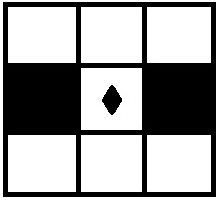
\includegraphics[scale=0.6]{ej3/imgs/ejSinSolucion.png}

Es imposible colocar sensores de forma tal que el casillero importante sea apuntado por dos sensores ya que de ninguna manera se puede lograr que sea apuntado de forma horizontal por la presencia de las paredes. Removiendo alguna de las paredes obtenemos una grilla en la cual se puede obtener una solución:

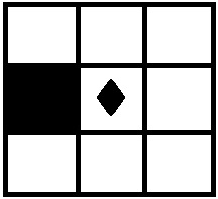
\includegraphics[scale=0.6]{ej3/imgs/grillaConSolucion.png}

Una solución posible para esta configuración es la siguiente:

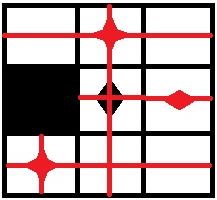
\includegraphics[scale=0.6]{ej3/imgs/solValidaPeroNoOptima.png}

Sin embargo esta solución no es óptima ya que el costo total es de \$16000 (dos sensores cuatridireccionales y uno bidireccional) y es posible encontrar una mejor:

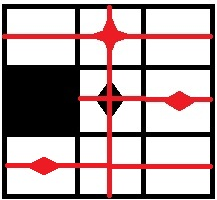
\includegraphics[scale=0.6]{ej3/imgs/solOptima.png}

Aquí el costo es de \$14000 (dos sensores bidireccionales y uno cuatridireccional).


